\section{Discussion}
\label{Sec:discussion}

% \head{Correlation.} To examine the relationship between the 
% cyclomatic complexity of objects and the number of unique invariants, 
% we used R \cite{?} to calculate the non-parametric
% Spearman correlation coefficients (r) as well as the p-values (p), 
% and plotted the graphs. We present the combinations that
% indicate a possible correlation.\figref{inv-cc} depicts the scatter plot of the
% cyclomatic complexity versus the number of unique invariants. 
% The correlation coefficient ($r = 0.867$, $p = 0.002$) suggests that variables 
% are positively co-related: The higher the cyclomatic complexity, the more unique invariants
% are detected in the application. The reason might be that larger value of cyclomatic complexity 
% implies that more number of decision points are present in the program. Consequently, pushing more 
% restrictions on varibales and parameters of the application may result in inferring more number of
% invariants. 
% \begin{figure}
% \centering
% 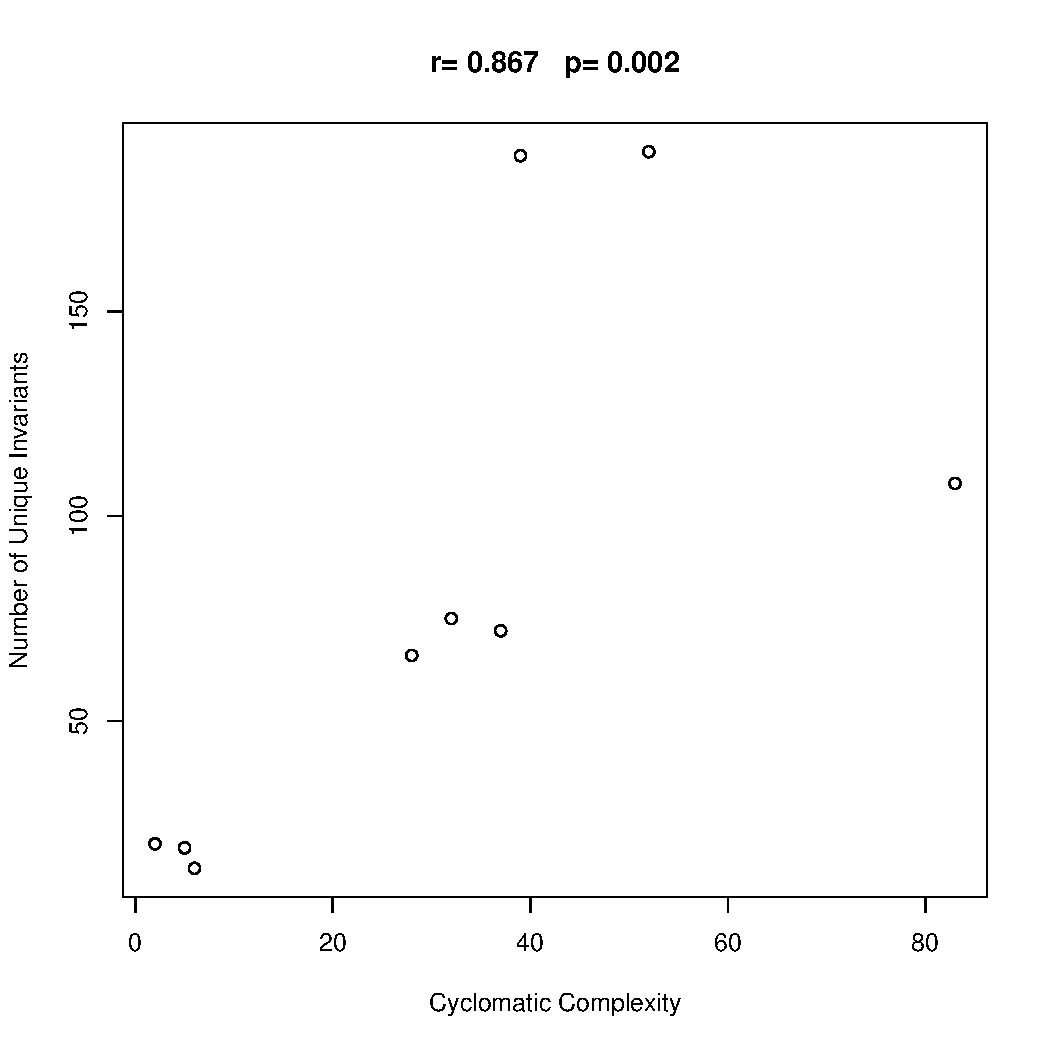
\includegraphics[width=0.7\hsize]{rscripts/inv_cc}
% \mycaption{Scatter plot of the number of unique invariants versus
% cyclomatic complexity. r represents the Spearman correlation coefficient and p is
% the p-value.}
% \label{Fig:inv-cc}
% \vspace{-0.3in}
% \end{figure}
%(1) the precision of comparing two floating point numbers in Daikon;
%The first is concerned with the number of digits in the fractional part of the floating point numbers, which is used by Daikon while comparing two floats. We resolve this by increasing the precision of float comparisons in Daikon configurations.
\head{Unstable Assertions.} As mentioned in \secref{filtering}, we observe a few number of unstable invariant assertions initially, which are removed by our filtering mechanism. By analyzing our trace data, we observe
that such unstable assertions arise mainly because of the 
multiple runtime types of \javascript variables.
This is based on the fact that in \javascript it is possible to change the type of a variable at runtime. However, Daikon treats variables as single type, selects the first observed type, and ignores the subsequent types in the trace data. This results in producing a few number of unstable invariant assertions for \javascript.
We remove such unstable assertions in our filtering step. A drawback of removing these assertions, is that our tool might miss a fault during the regression testing phase.
However, according to our observations, such unstable assertions form only around 5\% of the total generated assertions. Thus, we are still able to achieve high accuracy as presented in the previous section.
    
\head{Limitations.} Our approach is not able to detect syntax errors that are present in the \javascript code. Furthermore, tracing DOM manipulations using APIs other than the standard DOM API or jQuery is currently not supported by \jsart.
Further, a regression fault either directly violates an invariant assertion, or it can violate closely 
related assertions, which have been affected by the fault. However, if the tool is not able to infer any invariants in the  affected scope of the error, it fails to detect the fault. This results in observing a low rate of false negatives as illustrated in \secref{evaluation}. 
     
\head{Revisiting the Assumptions.} As we mentioned in \secref{approach}, we assume that the current version of the web application is bug-free. This is based on the fact that in regression testing a gold standard is always needed as a trusted version for comparing the test results against \cite{Binder:2000} to detect regression faults. However, if the original version of the application does contain an error, the generated assertions might reflect the error as well, and as such they are not able to detect the fault. 
Our second assumption states that the program specifications are unlikely to change frequently in revisions. Here we assume that software programs evolve gradually and regression faults are mostly due to small changes. However, if major upgrades occur in subsequent revisions such that the core specification of the application is affected, the inferred invariants from the original version may not be valid any longer and new invariant assertions need to be generated.

% Competent Programmer Hypothesis (CPH) \cite{acree:mutation1979, demillo:computer1978}. It states that programmers tend to develop programs, which are close to the correct version. Therefore,
% regression faults are mostly due to simple faults occur during small changes in the program. These faults made by competent programmers are merely simple faults such that the applications's behavior is not significanlty affected.


 

\begin{table}[t]
%\vspace{5pt}
        \caption{Manual effort imposed by our approach for deriving stable invariant assertions.}
{\scriptsize
    \begin{center}
       
      %  \subtable[Experimental subjects and the corresponding exploration data]
            {
           \begin{tabular}{c|c|c} \hline
\thead{App ID} & \thead{Total Time (min)} & \thead{Manual Effort (min)} \\  \hline \hline

1  & 13  & 4 \\ \hline %535
           
2  & 11.5 & 3 \\ \hline %502

3 & 15.5  & 5 \\ \hline % 639

4  & 11  & 3 \\ \hline %500

5  & 6.5 & 2.5 \\ \hline %227

6  & 9  & 4.5 \\ \hline %214

7  & 7.5  & 3.5 \\ \hline %244

8  & 6.5  & 2 \\ \hline %278

9  & 18 & 13 \\ \hline %266
\hline\end{tabular}\centering
            }
\label{Table:manualEffort_table}
\end{center}
}  
\vspace{-0.2in} 
\end{table}



\head{Automation Level.} While the testing phase of \jsart is fully automated, the navigation part requires some manual effort. Although the crawling is performed automatically, we do need to manually setup the tool with different crawling configurations per application execution.  Moreover, for each application run, we manually look at the size of the invariant output to decide whether more execution traces (and thus more crawling sessions) are needed.
%Thus, manual effort is concerned with tracing and filtering unstable invaraint assertions, where we need to execute the application 
%per crawling configuration. 
%
We present the manual effort involved with detecting stable invariant assertions in \tabref{manualEffort_table}. 
The table shows the total time, which is the duration time of deriving stable assertions including both automatic and manual parts. 
The reported manual effort contains the amount of time required 
for setting up the tool as well as the manual tasks involved with the navigation part.
The results show the average manual effort is less than 5 minutes.




